% !TeX root = ../libro.tex
% !TeX encoding = utf8

\chapter{El ciclo del litio}\label{ch:segundo-capitulo}

\section{Introducción}
La abundancia de litio observada en la fotosfera de las estrellas es un indicador de su composición interior y de los procesos de mezclado que en él tienen lugar. Adicionalmente, estas abundancias (además de otras métricas) se utilizan para comprobar la validez de los modelos estelares. Para que esto sea posible hay que tomar como premisa inicial que la abundancia de Litio generada en la nucleosíntesis asociada al Big Bang es conocida, y que este elemento solo se destruye a través de reacciones nucleares.\par 

En el ámbito de la astrofísica, persiste un enigma que desafía décadas de investigación teórica: las discrepancias entre los modelos de evolución estelar y las mediciones de abundancia de litio en estrellas. Estas discrepancias se manifiestan en estrellas que pertenecen a cúmulos de diferentes edades y que se encuentran en el mismo estado evolutivo, ya sea en la presecuencia principal (Pre-Main Sequence, PMS) o en la secuencia principal (Main Sequence, MS). A pesar de los esfuerzos, los modelos actuales no logran explicar las abundancias observadas en las etapas tardías de la MS \citep{Tschape2001}.\par

Es sabido que parte de la pérdida de litio se produce durante la PMS y que además ésta se acentúa según decrece la masa de la estrella y, a igualdad de masa, según aumenta la metalicidad de la misma. Para reproducir la dependencia entre la edad y masa de las estrellas con la merma de las concentraciones de litio, estos modelos necesitan de una combinación de procesos de mezclado cada vez más complejos, como rebasamiento (overshooting), mezclado debido a procesos rotacionales o difusión microscópica, o la presencia de campos magnéticos.\par

En la presente tesis estamos interesados en investigar cómo la presencia de campos magnéticos pueden influir en las abundancias de litio detectadas en las atmósferas de las estrellas de tipo solar. El litio es un elemento que se destruye fácilmente en las capas interiores de este tipo de estrellas. Este proceso ocurre principalmente durante la PMS en mayor medida, aunque puede darse también durante la MS. Adicionalmente, cabe la posibilidad de que se dé en las capas exteriores si existe un proceso eficiente de mezclado en la estrella, en el que puede influir la presencia de campos magnéticos. Por tanto, el estudio de la abundancia de litio en la superficie de la estrella puede ser clave para entender el proceso de evolución del momento angular de la misma.\par

\section{El litio primordial}
Los modelos teóricos existentes de evolución estelar no informan sobre la cantidad inicial de litio que tiene una estrella, sólo describen cómo se agota. Por tanto, para hacer una estimación precisa de la abundancia inicial de litio, es un requisito poder comparar previamente las observaciones y los modelos. Nuestro Sol representa una excepción única, ya que nos permite conocer la abundancia actual de este elemento en su fotosfera, $A(\isotope[7]{Li}) = 1.1 \pm 0.1 \, dex \footnote{Contracción procedente del inglés para decimal exponent.}$ \citep{Jeffries2004}, donde $A(\isotope[7]{Li})$ se define según la Ecuación \ref{eq:A_Li}

\begin{ceqn}
	\begin{equation}
		A(\isotope[7]{Li}) = log\frac{N(Li)}{N(H)} + 12
		\label{eq:A_Li}
	\end{equation}
\end{ceqn}

donde $N$ es el número de átomos del elemento en cuestión por unidad de volumen y 12 representa la abundancia de $H$, el cual se toma como punto de referencia para evitar que aparezcan números negativos.\par

Por otro lado, la abundancia inicial de $A(\isotope[7]{Li}) = 3.34$ dex se obtiene a partir de mediciones de meteoritos \citep{Randich2006}. Según la teoría establecida para las estrellas recién nacidas, tenemos que la abundancia inicial de litio puede estimarse con bastante precisión a partir de mediciones fotosféricas en estrellas de tipo T-Tauri, o de las estrellas F más calientes que forman parte de cúmulos algo más antiguos. Para estas últimas, la teoría actual de la evolución estelar sugiere que el litio aún no debe estar agotado. Los resultados obtenidos a partir de las medidas en ambos tipos de estrellas nos permiten fijar la abundancia inicial de litio en el intervalo $3.0 < A(\isotope[7]{Li}) < 3.4$ dex \citep{Randich2006}.\par


\section{Evolución del litio en la presecuencia principal (PMS)}
La PMS es la continuación directa de la fase protoestelar. Inicialmente, a medida que el objeto estelar joven evoluciona a lo largo del tiempo, su luminosidad es fundamentalmente consecuencia directa de un proceso de acreción suficientemente fuerte que es capaz de mantener la fusión activa de deuterio \citep{Stahler1983}. Una vez que cesa la acumulación de material, la protoestrella, rodeada sólo por un disco residual de material, desciende a lo largo de su traza de Hayashi de una forma casi vertical. Esta fase de la evolución estelar se localiza en el diagrama Hertzspring-Russell (HR) \footnote{Diagrama en el que se enfrenta la luminosidad de la estrella contra su temperatura} y en la misma la estrella es totalmente convectiva. A medida que la estrella desciende por la traza de Hayashi se va contrayendo y su radio disminuye, a la par que lo hace su luminosidad. Su temperatura superficial ($\teff$) tiende a mantenerse  en torno $3000..5000$ K aunque ésta va en aumento a consecuencia de la contracción del gas que conforma la estrella y el aumento de presión. Llegado un punto con suficiente temperatura en el interior de la estrella, ésta desarrolla una zona convectiva y la estrella entra en la traza de Heney, donde se producen reacciones nucleares, marcando así la entrada en la MS. \par

Durante la evolución estelar en esta fase, el Li se quema a temperaturas relativamente bajas ($2.5..3.0 \, 10^{6}$ K) y, en las estrellas de baja masa (< 1.2 $\msun$), el mezclado que se produce en la zona convectiva de la estrella puede hacer que el material ya agotado de litio alcance, en relativamente poco tiempo, la fotosfera de la estrella. Por esta razón, las mediciones de abundancia de litio fotosféricas nos brindan uno de los pocos métodos de sondeo de interiores estelares y, a su vez, representan un importante banco de pruebas contra el que enfrentar los resultados que se obtienen a partir de los modelos evolutivos para estrellas que se encuentran en la PMS. Entender cómo se produce el agotamiento del litio durante esta fase evolutiva también nos ofrece la posibilidad de poder estimar la edad de las estrellas más jóvenes y, por supuesto, es un punto de partida para poder cuantificar cualquier agotamiento subsiguiente de litio que se produzca a lo largo de la MS.\par

\begin{figure}
	\centering
	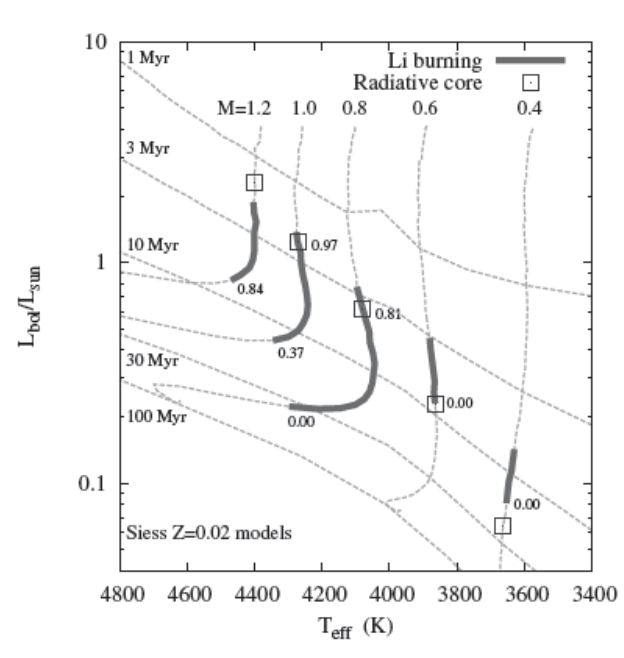
\includegraphics[width=0.5\textwidth]{img/tesis/isochrones.pdf}
	\caption {Secuencias evolutivas (en $\msun$) e isócronas (en Myr) para estrellas de baja masa comprendidas entre 0.4 y 1.2 $\msun$ y metalicidad Z=0.02. Se indican las franjas temporales en las que se produce el agotamiento fotosférico de Li y el desarrollo de un núcleo radiativo. Los números a la derecha de los intervalos de destrucción de Li indican la fracción fotosférica de éste que queda en el punto donde se desarrolla el núcleo radiativo y al final de su combustión, figura de Jeffries (2004).}
	\label{fig:isocrhones}
\end{figure}

La Figura \ref{fig:isocrhones} muestra la fase PMS para modelos de distintas masas iniciales. Asimismo, se indican la fase de quema de litio y el momento de aparición del núcleo radiativo. Como se puede observar, las estrellas con una masa $\mstar$ < 0.35 $\msun$ que se encuentran en la PMS tienen una estructura relativamente sencilla: son totalmente convectivas hasta que consiguen alcanzar la edad de finalización de secuencia principal (Termination Age Main Sequence, TAMS). A medida que la estrella va reduciendo su volumen según desciende a lo largo de la traza de Hayashi, su núcleo se va calentando, pero el gradiente de temperatura se mantiene muy cerca del gradiente adiabático, el cual delimita la frontera entre un núcleo radiativo o convectivo. Esta situación se mantiene para la práctica totalidad de la estrella, con la excepción de las capas superficiales.\par 

El litio comienza a arder en reacciones de captura protónica cuando la temperatura central, $T_c=2.5 \, 10^{6}$ K y, debido a que la tasa de reacción es tan sensible a la temperatura para densidades típicas de PMS \citep{Randich2006} y a que el mezclado convectivo se produce de forma tan rápida, todo el litio se quema en una pequeña fracción de tiempo. Por otra parte, se ha contrastado que la edad a la que se produce el agotamiento de litio es inversamente proporcional a la masa de la estrella, es decir, aumenta según disminuye la masa hasta que se alcanza el límite de $\mstar$ < 0.06 $\msun$, ya que en este tipo de estrellas nunca llegará a alcanzarse una temperatura lo suficientemente alta como para poder quemar litio.\par

En las estrellas $\mstar$ > 0.35 $\msun$, el proceso de agotamiento del Li es bastante más complejo. Tienen densidades centrales más bajas y a medida que la $T_c$ aumenta durante la contracción del PMS, la opacidad cae lo suficiente como para que el gradiente de temperatura se vuelva subadiabático, es decir, inhibe el proceso de mezclado y se forma un núcleo radiativo que empuja hacia afuera para incluir una fracción rápidamente creciente de la masa estelar.  Para $\mstar$ <  $\msun$ solo existe una pequeña ventana de oportunidad en la que poder quemar un poco de litio antes de que se desarrolle el núcleo radiativo (aproximadamente a 2 Ma para 1 $\msun$). Como se puede observar en la Figura \ref{fig:isocrhones}, para $\mstar$ < 0.6 $\msun$ el núcleo radiativo se desarrolla antes de que la quema de litio esté completa. A falta de mezcla por convección, el material agotado de litio no puede llegar a la fotosfera y una vez que la temperatura en la base de la zona de convección cae por debajo del umbral de combustión de litio, el agotamiento de litio fotosférico se detiene. Para una estrella de 1 $\msun$, el agotamiento de litio fotosférico comienza aproximadamente a los 2 Ma y debería de terminar al alcanzar los 15 Ma.\par

Los estudios sobre el litio en los cúmulos muy jóvenes indican que las estrellas de tipo solar sufren muy poco (si es que lo hay) agotamiento de litio durante las fases de la PMS  \citep{Jeffries2004}. Al mismo tiempo, se ha dedicado una gran cantidad de esfuerzo observacional al muestreo de abundancia de litio y también del berilio \citep{Mena2011, DelgadoMena2014} con el objetivo de poner restricciones empíricas más severas a los mecanismos propuestos.\par

\section{Evolución del litio en la secuencia principal (MS)}
Como ya mencionaron \cite{Zappala1972} en su trabajo hace más de cinco décadas, la medición de litio en cúmulos más antiguos que los Hyades es una herramienta clave para investigar el agotamiento que sufre el litio en la MS, además de las escalas de tiempo en las que ocurre este proceso. Tres décadas después, se realizaron nuevas mediciones de litio para varios cúmulos antiguos, incluyendo NGC 752 y M 67 \citep{Sestito2006} que permitieron caracterizar de manera más completa la dispersión de litio en estrellas de tipo solar y con metalicidad y edad similar al Sol \citep{Sestito2005}. Recientemente, gracias a los datos aportados por el satélite Gaia \citep{Brown2016, Brown2018, Brown2021, Brown2022} y a las abundacias de litio obtenidas a partir de ellos por el estudio Gaia ESO (Gaia ESO Survey, GES) \citep{Gilmore2012,Randich2013,Randich2022} tenemos a nuestra disposición un mayor volumen de datos que nos permiten refinar aun más nuestros modelos.\par

Basándonos en los resultados de los modelos de evolución estándar que solo tienen en cuenta los procesos de convección como los mecanismos a través de los cuales se produce el mezclado, solo debería agotarse el litio en la PMS, ya que es en esta fase cuando las estrellas exhiben una envolvente convectiva profunda con una base lo suficientemente caliente como para quemar el litio. Por otra parte, estos mismos modelos predicen que este proceso se detiene en la MS para estrellas de tipo solar o aquéllas más calientes. Sin embargo, los estudios llevados a cabo con cúmulos abiertos han revelado abundancias de litio A(Li) 10 veces inferior respecto a los valores esperados en estrellas en su MS \citep{Sestito2005}, y de hecho, nuestro propio Sol presenta un agotamiento una A(Li) 100 veces inferior si la comparamos con la detectada en los meteoritos \citep{Lodders2003}.\par

\begin{figure}
	\centering
	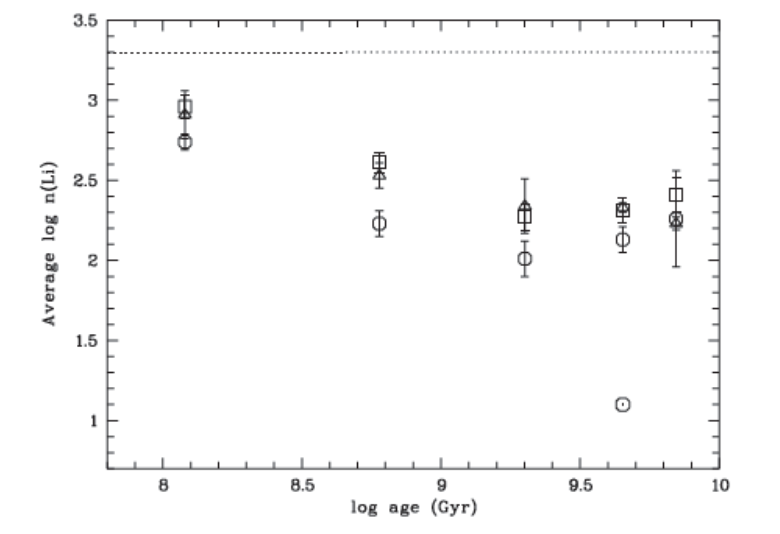
\includegraphics[width=0.5\textwidth]{img/tesis/li_abundances_vs_age.pdf}
	\caption{Abundancia media de litio en función de la edad. Las masas y edades han sido estimadas a partir de las temperaturas efectivas hacienda uso de isócronas. Las abundancias de litio se denotan mediante la notación log n(Li) = N (Li)/N (H) + 12. Los diferentes símbolos indican estrellas con diferentes masas, a saber: 1$\pm$0.02 $\msun$ (círculos), 1.05$\pm$0.02 $\msun$ (cuadrados) y 1.1 $\pm$0.02 $\msun$ (triángulos). El Sol ($\odot$) también se muestra. La línea horizontal indica la abundancia primigenia de litio, figura de \cite{Randich2006}.}
	\label{fig:li_abundances_vs_age}
\end{figure}

La Figura \ref{fig:li_abundances_vs_age} muestra que la evolución del litio desde aproximadamente 100 Ma hasta 6-8 Ga es similar para los 3 rangos de masas. Se observa que los valores log n(Li) declinan a una ratio casi constante a medida que la estrella envejece. Esto ocurre así hasta aproximadamente los 2 Ga, momento a partir del cual el agotamiento del litio parece virtualmente detenerse y las abundancias tienden a converger hacia los valores del Spite plateau, la línea de base en la A(Li) encontrada para estrellas antiguas (o de población II) y que por tanto se formaron a partir de material no alterado por otros procesos, que orbitan el halo galáctico. \par

\section{Mecanismos de destrucción de litio}
En este apartado procedemos a enumerar las diferentes opciones que actualmente defienden las principales líneas de investigación para intentar establecer una relación causa-efecto para la discrepancia de la abundancia de litio detectada en las fotosferas de estrellas de tipo solar.\par

\subsection{Litio y metalicidad}
Durante las últimas décadas, las estrellas con baja metalicidad ([Fe/H] < -1.0 dex), también denominadas de Población II, se han caracterizado por exhibir una relación bastante estable entre la abundancia de litio y su metalicidad \citep{Guiglion2016}. Este nivel quedó inicialmente vinculado a la abundancia primordial asociada al litio, aunque esta situación cambió a la luz de los resultados obtenidos por la misión de la sonda de anisotropía de microondas Wilkinson (Wilkinson Microwave Anisotropy Probe, WMAP), que propiciaron que la abundancia de este elemento predicha por el modelo estándar de nucleosíntesis para el Big Bang (Standard Big Bang Nucleosynthesis, SBBN) pasara a estimarse en 2.6 dex \citep{Spergel2003}. Este dato, sin embargo, entra en contradicción con la abundancia de litio medida en enanas viejas de baja metalicidad  (A(Li) $\simeq$ 2.2 dex) situadas en el halo de la galaxia conocido como el Spite plateau \citep{Spite1982}. Además, para estrellas de baja metalicidad (ver Figura \ref{fig:li_abundances_sbbn}) se ha encontrado que la abundancia de litio no parece guardar relación con la metalicidad de la estrella \citep{Fu2015}.\par


\begin{figure}
	\centering
	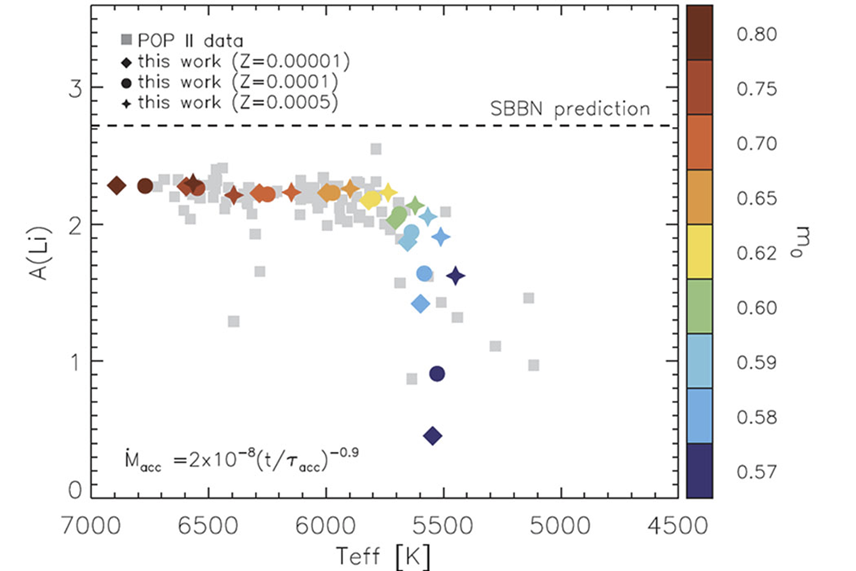
\includegraphics[width=0.5\textwidth]{img/tesis/li_abundances_sbbn.pdf}
	\caption{La abundancia de litio derivada para estrellas de baja metalicidad situadas en la secuencia principal es aproximadamente tres veces menor que el valor de litio primordial predicho por la SBBN, figura de \cite{Fu2015}.}
	\label{fig:li_abundances_sbbn}
\end{figure}

Se han realizado investigaciones para intentar vislumbrar si existe una relación entre las concentraciones de litio y la metalicidad de la nube de la que surgen las estrellas \citep{Pinsonneault1997, BarradoyNavascues2001}). Parece que esto no es así y el agotamiento del litio observado no sugiere que dependa de manera concluyente del contenido en elementos metálicos presente en esa nube primordial \citep{Guiglion2016}. Adicionalmente, se ha contrastado que tanto para los cúmulos jóvenes (alta metalicidad) como para los antiguos (baja metalicidad), cuyos niveles de metalicidad varían aproximadamente $\pm$0.2 dex con respecto a la metalicidad de nuestro Sol, parecen compartir una distribución de litio muy similar \citep{Sestito2005}. Asímismo, se ha medido que la abundancia de litio medida en el Sol es mucho más baja que la que presentada por otras estrellas similares situadas en su vecindad \citep{Reddy2003}. Esta variación es más acusada que la detectada para otros tipos de elementos presentes en él.\par

Por otro lado, otros autores \citep{Sestito2005} defienden que la amplia gama de abundancias de litio observadas en estrellas similares al Sol y cercanas a éste es más fácilmente explicable si se establece una dependencia entre la abundancia de Li, la edad y masa de la estrella.\par

A la luz de los resultados y conclusiones expuestas en los diferentes trabajos, se hace evidente que no existe un consenso unánime sobre la posible relación entre la metalicidad de una estrella y su abundancia de litio.\par

\subsection{Litio y convección}
Una gran cantidad de trabajo teórico y observacional se ha dedicado a la comprensión de litio y su evolución. Aún así, las evidencias acumuladas no terminan de concordar con las predicciones de los modelos estándar \citep{Sestito2005}; entendiendo por estándar a aquellos modelos que incluyen sólo los mecanismos de convección como proceso de mezcla y no tienen en cuenta fenómenos que podrían influir también como el transporte, como la difusión, las ondas de gravedad (nos referimos a ondas en el fluido de la estrella inducidas por la gravedad), la pérdida de momento angular o la presencia de planetas.\par

En las estrellas de tipo solar, la quema de litio se produce a una temperatura aproximada de $2.5 10^{6}$ K mediante las reacciones de captura protónica que acontecen en interiores estelares. Por lo tanto, si se mantiene de manera continuada en el tiempo el mecanismo que transporta el litio entre la zona de convección exterior químicamente mixta y las regiones más profundas que poseen temperaturas lo suficientemente altas, éste acabará siendo destruido y su abundancia fotosférica disminuirá, llegando en algunos casos prácticamente a desparecer de la superficie estelar \citep{DelgadoMena2014}.\par

A su vez, la abundancia de litio medida en la fotosfera nos sirve también para realizar la calibración de modelos de evolución estelar. Sin embargo, es preciso mencionar que para que este planteamiento sea coherente, hay que suponer que la abundancia inicial de litio es conocida y que éste es única y exclusivamente destruido mediante reacciones nucleares.\par

\subsection{Litio y difusión}
Un factor determinante para conocer la fase evolutiva en la que se encuentra una estrella es su composición química interna. Los modelos estándar consideran, como hemos apuntado anteriormente, a los procesos desencadenados por reacciones nucleares y por convección como los únicos que pueden modificar este perfil químico. Sin embargo, la difusión química de elementos también puede alterar este perfil y puede considerarse como otro mecanismo que contribuye a la disminución de la abundancia de litio en la superficie que tiene lugar a lo largo de MS. Este sería otro factor a tener en cuenta que contribuiría a poder explicar por qué la abundancia solar fotosférica es mucho menor que la meteórica. Sin embargo, este proceso estelar a largo plazo no puede ser observado directamente en las estrellas.\par

En el trabajo de \cite{Richard2004} mostraron que la menor abundancia de litio observada en las estrellas de tipo Población II es el resultado del agotamiento del mismo producido por el efecto de difusión atómica que entra en competencia con los procesos de mezclado en las zonas radiativas de estas estrellas.La difusión microscópica acorta la vida útil de la secuencia principal y conduce a un agotamiento de los elementos superficiales. El modelo solar requiere de su inclusión o de lo contrario ni siquiera la edad del Sol se podría producir correctamente \citep{Thoul1993}.\par

\subsection{Litio y exoplanetas} \label{sec:litio_exoplanetas}
El descubrimiento de un gran número de exoplanetas durante las dos últimas décadas \citep{Mayor1995, Bonfils2018} ha significado un importante empuje para la comunidad científica en el campo de la astrofísica. Aparte de las consecuencias directas derivadas de poder estudiar los nuevos planetas descubiertos más allá de nuestro sistema solar, lo que ya es de por sí extremadamente interesante, no lo es menos la observación de sus estrellas anfitrionas, ya que éstas pueden llegar a aportar información muy valiosa acerca de las características globales, composición y formación de los sistemas planetarios extrasolares que albergan.\par

La hipótesis de que la variabilidad de concentración de litio en las estrellas puede ser debida a una posible correlación entre la presencia de planetas es una línea de trabajo de diversos estudios \citep{Israelian2009, DelgadoMena2014, Figueira2014}. Estas investigaciones apuntan a que esta presencia podría ser el desencadenante de la discrepancia en la abundancia de litio medidas en estrellas de tipo solar. Para nuestro Sol, ésta es unas 140 veces inferior a la que le correspondería a su modelo estelar \cite{Israelian2009}, aunque la temperatura en en el límite inferior de la zona convectiva (Bottom Convective Zone, BCZ) no es lo suficientemente alta como para quemarlo.\par

En un primer momento, esta línea de investigación no se encontraba suficientemente fundamentada en evidencias que apoyasen este planteamiento, y esto se debía a la escasa disponibilidad de datos sobre estrellas que tuviesen sistemas planetarios asociados. En los últimos años, gracias a satélites como CoRoT \cite{Baglin2006} y Kepler \cite{Borucki2010}, dedicados a la búsqueda de planetas extrasolares, se han podido obtener datos de un gran número de estrellas con sistemas planetarios asociados. Esta nueva situación ha derivado en la realización de nuevos trabajos, o en la revisión de otros anteriores, en los que se han podido realizar nuevos estudios comparativos más amplios y sin sesgo en lo que se refiere a poder comparar estrellas con y sin sistemas planetarios. Estos nuevos trabajos han arrojado evidencias, tanto a favor \citep{Bouvier2008, Israelian2009} como en contra \citep{Baumann2010}, sobre la existencia de una relación directa entre la menor abundancia de litio en las estrellas con planetas con respecto a las que no tienen.\par

Respecto a los primeros, la línea argumental postula que la presencia de planetas alrededor de una estrella podría afectar la evolución de la abundancia de litio fotosférico al afectar historia rotacional de su estrella anfitriona. Mediante el desarrollo de modelos de evolución de tipo solar incluyendo rotación, tanto para rotadores lentos (unas 5 veces mayor la velocidad de rotación del Sol) como rápidos (unas 70 veces mayor), que se hacen evolucionar desde la PMS hasta la edad actual de nuestro Sol, han conseguido encontrar pruebas de que las estrellas con una rotación menor desarrollan un alto grado de rotación diferencial entre el núcleo radiativo y la envolvente convectiva, mientras que los rotadores rápidos evolucionan con poco desacoplamiento entre núcleo y envoltura. A raíz de esta fuerte rotación diferencial en la base de la envoltura convectiva, en los rotadores lentos el proceso de destrucción del litio se vuelve más eficiente, concluyendo que las estrellas que albergan exoplanetas y presentan un agotamiento del litio debieron de ser rotadores lentos durante ZAMS y que esto se debió a una interacción duradera entre la estrella y el disco plotoplanetario durante la PMS. Esto se ve reforzado por análisis comparativos realizados entre estrellas que algerban planetas y otras que no. En la Figura \ref{fig:li_abundances_planets} podemos observar como la gran mayoría de aquéllas que poseían planetas presentaron una disminución acusada en la abundancia de litio respecto de las que no tenían planetas.\par

Entre los que apuntan a que no existe relación directa alguna entre la menor abundancia de Li detectada en la atmósfera de las estrellas que albergan planetas y las que no los tienen, se argumentación radica en el hecho de que las evidencias encontradas por otros investigadores en la dirección de la existencia de una relación entre las abundancias de litio detectadas y las estrellas que albergan planetas, se deben única y exclusivamente a consideraciones sesgadas y errores sistemáticos producidos durante el análisis de los datos recopilados. Por el contrario, estos mismos autores sostienen que sí existen evidencias claras entre la abundancia de litio de una estrella con su edad y la metalicidad (Z) de la misma. Por otra parte, la ingestión de un planeta “fallido” podría ser la causa por la que se produce un aumento de la abundancia de este elemento en la superficie de las estrellas.\par

\begin{figure}
	\centering
	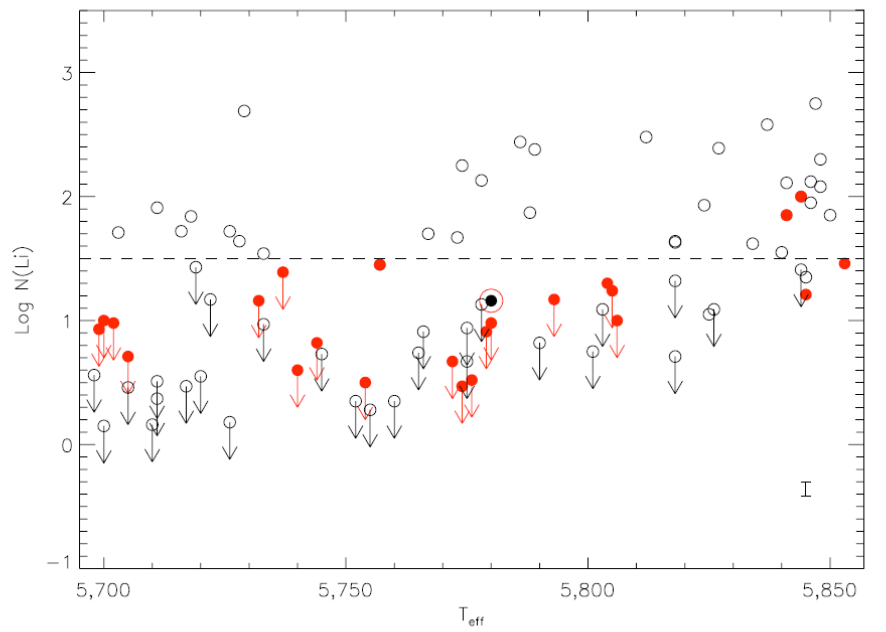
\includegraphics[width=0.5\textwidth]{img/tesis/li_abundances_planets.pdf}
	\caption{Abundancia de litio vs temperatura efectiva en estrellas de tipo solar con y sin planetas. Las estrellas con planetas vienen representadas por los círculos rojos y las sin planetas por los círculos vacíos. El Sol queda representado por el punto negro rodeado de un círculo rojo, figura de \cite{Israelian2009}.}
	\label{fig:li_abundances_planets}
\end{figure}


\subsection{Litio y rotación}
El impacto de la rotación tanto en la PMS como en el agotamiento del Li para las estrellas de tipo solar ha sido ampliamente debatido en el pasado \citep{Pinsonneault1997,Jeffries2004,Somers2014} y revisado más recientemente sobre la base de la disponibilidad de medidas más precisas \citep{Bouvier2016}. Los resultados sugieren una conexión entre la velocidad de rotación de las estrellas y la abundancia de litio detectada en sus atmósferas estelares, de modo que las estrellas que giran más rápido destruyen menos litio que las que lo hacen de manera más lenta. De alguna manera los resultados publicados por \cite{Bouvier2016} son inesperados ya que apuntan en una dirección diametralmente opuesta a los de trabajos anteriores, en los que se predecía que las estrellas que rotan más rápidamente deberían de destruir una mayor cantidad de litio.\par 

Para explicar esta tendencia, es necesario recurrir a mecanismos adicionales que vinculen el agotamiento del litio y la rotación. Esta aparente contradicción de los resultados de diferentes trabajos no tiene por qué se tal. De hecho se plantean diferentes ideas que pueden ayudar a entender las discrepancias, entre las que se encuentra el acoplamiento de las estrellas con sus disco proto-estelar (ver \ref{sec:litio_exoplanetas}), que influiría en los mecanismos de mezclado ocasionados por la rotación \citep{Bouvier2008, Eggenberger2012}, la influencia de campos magnéticos \citep{Eggenberger2009} que tienen la propiedad de transmitir el momento angular (AM) de forma mucho más eficaz que inducir la mezcla \citep{Denissenkov2007}. Como consecuencia de este incremento en la eficiencia del transporte del AM, se reduce la cantidad de rotación diferencial entre las zonas radiativa y convectiva de la estrella (se fomenta una rotación de cuerpo sólido), así como las inestabilidades rotacionales inducidas. La acreción de material \citep{Baraffe2010} también se postula como una posibilidad para explicar la menor abundancia de litio para estrellas en el mismo rango de masas y edad. Episodios periódicos de acreción de material por parte de la estrella conducen a desarrollar temperaturas centrales significativamente más altas. A consecuencia de ello, una mayor cantidad de litio puede ser destruido.\par


\subsection{A qué se debe esta merma de litio}
Como hemos enumerado en las secciones anteriores, existe una propuesta amplia de potenciales mecanismos que podrían, por una parte, gobernar el ciclo de vida del litio, y por otra, ayudar a entender a qué se deben las discrepancias entre las observaciones y los resultados arrojados por los modelos. Sirva como ejemplo la línea de trabajo de \cite{Ramirez2012} en el que sus autores miden las abundancias de litio de una gran muestra de estrellas para encontrar correlaciones entre éstas y otras propiedades. Tales correlaciones deberían poder ayudar a determinar exactamente cómo se destruye el litio en las estrellas y cómo la abundancia galáctica de este elemento ha cambiado durante la vida de la Vía Láctea.\par 

De manera genérica, estos mecanismos pueden agruparse en dos ideas principales. Por un lado, los que abogan por la propuesta de que la abundancia de este elemento en la superficie de las estrellas podría ser menor de la que los modelos predicen debido a que el litio podría haberse transformado en elementos más pesados mediante reacciones nucleares. El mayor inconveniente de este planteamiento es que la temperatura requerida para fusionar el litio y crear otros elementos es normalmente más elevada que la que puede ser alcanzada por las capas externas convectivas presentes en estrellas similares a nuestro Sol. Por esa razón, se ha propuesto una segunda explicación alternativa que plantea que el litio podría haberse mezclado en las capas más profundas de la estrella y de este modo, haber desaparecido de las zonas exteriores \citep{Pinsonneault1997}.\par



\section{El litio y las reacciones nucleares} \label{sec:li_reac_nuc}
Hasta aquí hemos presentado los posibles mecanismos que influyen de manera más o menos directa en la destrucción del litoi, pero finalmente éste se destruye porque se produce una "quema" del mismo cuando las condiciones en el interior estelar son las adecuadas para que se produzcan una serie de reacciones nucleares. Como consecuencia, para poder obtener las abundancias de litio al final de la TAMS, primeramente necesitamos conocer qué reacciones nucleares son las responsables de su creación. De acuerdo a Cox y Giuli \citep{Cox1968}, en las condiciones de temperatura y densidad que se dan en el interior de una estrella de tipo solar (1.0 $\msun$), el tiempo de vida de los elementos más ligeros: $\isotope[2]{H}$, $\isotope[3]{H}$, $\isotope[6]{Li}$, $\isotope[9]{B}$, $\isotope[10]{B}$ y $\isotope[11]{B}$ y los resultantes de combinarse con el H a través de las reacciones de cadena protón-protón en sus variantes I, II y III, tienen un tiempo de vida que va desde los pocos segundos hasta los aproximadamente $10^4$ años. Por lo tanto, todos estos elementos deberían de consumirse en las etapas iniciales de vida de la estrella, tan pronto su interior ronde los $10^7$ K.\par

La cadena de reacción protón-protón I es la cadena de reacciones dominantes en estrellas de tamaño solar o menor. El primer paso conduce a la fusión de dos núcleos de hidrógeno $\isotope[1]{H}$ (protones) a deuterio $\isotope[2]{H}$, liberando un positrón y un neutrino al transformar un protón en un neutrón. El positrón resultante de dicha reacción se aniquila inmediatamente con un electrón y su masa se convierte en energía liberada a través de dos fotones gamma. Tras esta reacción, el deuterio producido en el primer paso se puede fusionar con otro hidrógeno para producir un isótopo ligero de helio $\isotope[3]{He}$. A partir de este punto la reacción se subdivide en tres ramas diferentes que desembocan todas en la generación de un núcleo $\isotope[4]{He}$. En la variante I (Figura \ref{fig:pp-I}), éste se produce por la fusión de dos núcleos de $\isotope[3]{He}$.\par


\begin{figure}
	\centering
	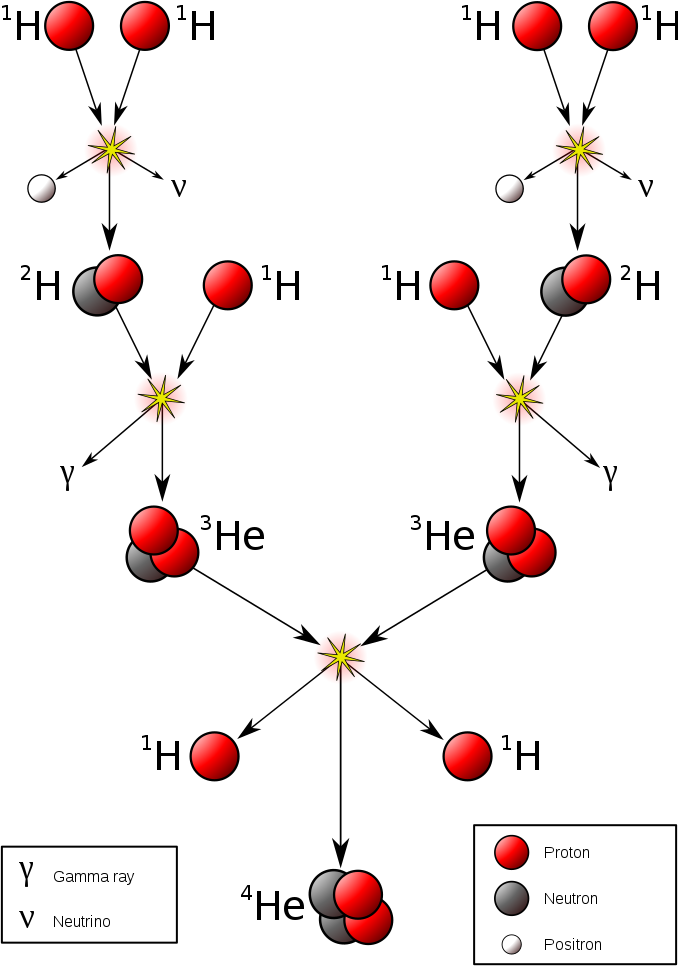
\includegraphics[width=0.35\textwidth]{img/tesis/pp-I.png}
	\caption {Cadena de reacciones protón-protón I (pp-I)}
	\label{fig:pp-I}
\end{figure}

En las otras dos variantes, II (\ref{fig:pp-II}) y III (\ref{fig:pp-III}), se requiere del $\isotope[4]{He}$ previamente producido y ambas cadenas surgen a consecuencia de los dos caminos que el $\isotope[7]{Be}$ puede tomar. Como podemos observar un primer paso en común para las tres cadenas es la fusión de dos protones en deuterio.

\begin{figure}
	\centering
	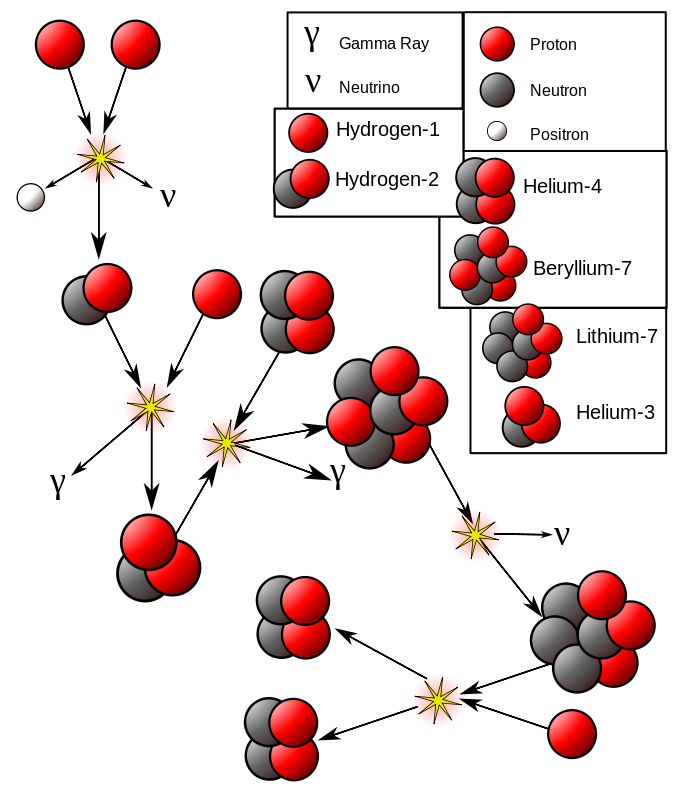
\includegraphics[width=0.35\textwidth]{img/tesis/pp-II.png}
	\caption {Cadena de reacciones protón-protón II (pp-II)}
	\label{fig:pp-II}
\end{figure}

De particular interés para este trabajo es la variante II, ya que en ella es donde se produce $\isotope[7]{Li}$. En esta variante de la reacción se requieren temperaturas del orden de $1.4x10^7..2.3x10^7$ K. Bajo estas condiciones los isótopos estables de $\isotope[3]{He}$ se fusionan con núcleos de $\isotope[4]{He}$ para dar lugar a $\isotope[7]{Be}$, que tras capturar un electrón forma $\isotope[7]{Li}$. Finalmente, $\isotope[7]{Li}$ se fusiona con un protón para dar lugar a dos núcleos de $\isotope[4]{He}$.\par

\begin{figure}
	\centering
	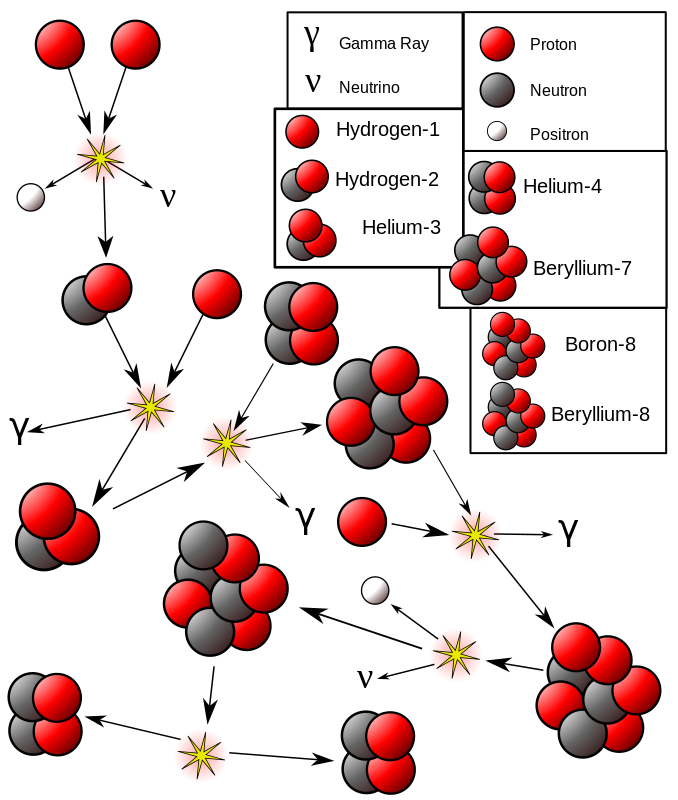
\includegraphics[width=0.35\textwidth]{img/tesis/pp-III.png}
	\caption {Cadena de reacciones protón-protón III (pp-III)}
	\label{fig:pp-III}
\end{figure}

La variante III es la rama dominante cuando se alcanzan temperaturas superiores a los $2.3x10^7$ K. En esta rama, el $\isotope[7]{Li}$ se fusiona con un protón para formar un núcleo de $\isotope[7]{Li}$, que se descompone en un núcleo de $\isotope[8]{Be}$ y un positrón. Luego, el $\isotope[8]{Be}$ se descompone en dos núcleos de $\isotope[4]{He}$.\par

Los tres tipos de variantes ocurren de manera simultánea en el interior de las estrellas, pero unas son más frecuentes que otras. De acuerdo a las investigaciones teóricas, parcialmente soportadas por las medidas de neutrinos procedentes del Sol, se calcula que el 86\% de las reacciones se corresponden con las de tipo I, un 14\% con la de tipo II, y solo un 0.02\% con las de tipo III \cite{Scholz2018}.\par

De manera similar, la vida media de los isótopos involucrados en el ciclo CNO (Figura \ref{fig:ciclo-cno}) al recombinarse con el H dominante en esas primeras etapas debería de rondar los $10^6$-$10^7$ años. Sin embargo, este ciclo de fusión a través del cual las estrellas también generan He a partir del H es más representativo de estrellas con una masa superior a 1.3 $\msun$.\par


\begin{figure}
	\centering
	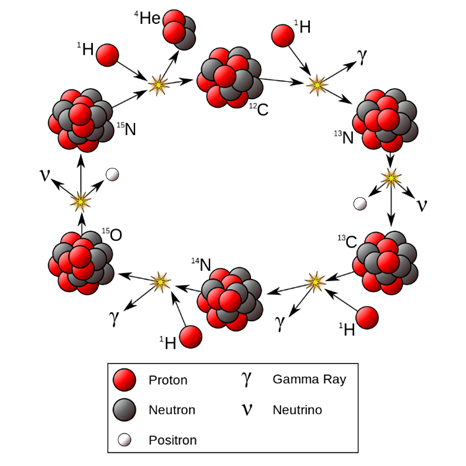
\includegraphics[width=0.4\textwidth]{img/tesis/ciclo CNO.png}
	\caption {Cadena de reacciones del ciclo CNO}
	\label{fig:ciclo-cno}
\end{figure}


\endinput
%--------------------------------------------------------------------
% FIN DEL CAPÍTULO. 
%--------------------------------------------------------------------
